\section{基坑支护结构专项施工方案}
\subsection{编制依据和工程概况}
\subsubsection{编制依据}

(1) 《建筑基坑支护技术规程》(JGJ120-2012)

(2) 《建筑桩基技术规范》(JGJ 94-2008)

(3) 《建筑基坑工程监测技术规范》(GB50497-2009)

(4) 《土层锚杆设计与施工规程》 (CECS22:90)

(5) 《深基坑工程施工安全技术规范》 JGJ311-2013

(6) 《混凝土结构设计规范》 GB50010-2015

(7) 《建筑结构静力计算手册》

\subsubsection{工程概况}

项目基坑开挖深度 10.0m,建筑周边环境良好,地下水水位 15m,对基坑的施工没有影响,本工程采用混凝土灌注桩加双层锚杆的支护方式,本工程所涉及的地层
共有三层,从上往下分别是:素填土 4m,粘土 6m,粉质黏土 10m,土层系数表详见表 \ref{tab:c6t1} 

\subsection{支护结构准备}
\subsubsection{灌注桩施工方案}

(1)施工顺序\\

平整场地→泥浆制备→埋设护筒→铺设工作平台→安装钻机并定位→钻进成孔→ 清孔并检查成孔质量→下放钢筋笼→灌注混凝土→拔出护筒→检查质量\\

(2)施工要点\\

\quan{1} 桩身混凝土强度等级不宜低于 C25

\quan{2} 支护桩的纵向受力钢筋宜选用 HRB400、HRB335 级钢筋,单桩的纵向受力钢筋不宜
少于 8 根,净间距不应小于 60mm

\quan{3} 箍筋可采用螺旋式箍筋,箍筋直径不应小于纵向受力钢筋最大直径的 1/4,且不应小于
6mm;箍筋间距宜取 100mm~200mm, 且不应大于 400mm 及桩的直径;

\quan{4} 纵向受力钢筋的保护层厚度不应小于 35mm

\quan{5} 锚拉式排桩或支撑式排桩,支护桩的桩径宜大于或等于 400mm;排桩的中心距不宜大于桩直径的 2.0倍。

\quan{6} 混凝土灌注桩采用沿桩截面周边非均匀配置纵向受力钢筋时,应按设计的钢筋配置方向
进行安放,其偏转角度不得大于 10°

\quan{7} 除特殊要求外,桩位的允许偏差应为 50mm;桩垂直度的允许偏差应为 0.5\%;预埋件位置的允许偏差应为 20mm;

\quan{8} 桩的其它施工允许偏差应符合现行行业标准《建筑桩基技术规范》 的规定

\begin{table*}
    \centering
    \caption{土层系数表}
    \label{tab:c6t1}
    \resizebox{\textwidth}{!}{
        \begin{tabular}{@{}llllllll@{}}
            \toprule
            序号 & 土层名称 & 厚度 h & 内摩擦角 $\phi$ & 粘聚力 c & 重度 & $K_a$ & $K_p$ \\ \midrule
            1 & 素填土  & 4.0m & 15\grad & 9 & 17.5 & 0.589 & 1.70 \\
            2 & 粘土 & 6.0m & 18\grad & 13 & 19.5 & 0.528 & 2.04 \\
            3 & 粉质黏土 & 10.0m & 20\grad & 18 & 19.6 & 0.490 & 1.89 \\ \bottomrule
            \end{tabular}}
    \end{table*}   


\subsubsection{锚杆施工方案}

(1)施工顺序\\

钻孔→锚杆安装→注浆→立锚墩→张拉→封孔注浆→外部保护\\

(2)施工要点\\

\quan{1} 锚拉结构宜采用钢绞线锚杆,且宜采用二次压力注浆工艺

\quan{2} 锚杆极限抗拔承载力应通过抗拔试验确定

\quan{3} 锚杆倾角宜取 15°~25°,且不应大于 45°,不应小于 10°

\quan{4} 锚杆的水平间距不宜小于 1.5m;多层锚杆,其竖向间距不宜小于 2.0m;

\quan{5} 锚杆腰梁应根据实际约束条件按连续梁或简支梁计算。计算腰梁的内力时,腰梁的荷
载应取结构分析时得出的支点力设计值

\quan{6} 型钢组合腰梁可选用双槽钢或双工字钢,槽钢之间或工字钢之间应用缀板焊接为整体
构件,焊缝连接应采用贴角焊。双槽钢或双工字钢之间的净间距应满足锚杆杆体平直穿过的要
求。

\quan{7} 当锚杆穿过的地层附近存在既有地下管线、地下构筑物时,应在调查或探明其位置、走
向、类型、使用状况等情况后再进行锚杆施工

\quan{8} 采用二次压力注浆工艺时,二次压力注浆宜采用水灰比 0.50~0.55 的水泥浆;二次注
浆管应牢固绑扎在杆体上,注浆管的出浆口应采取逆止措施;二次压力注浆时,终止注浆的压
力不应小于 1.5MPa;

\quan{9} 锚杆的钻孔深度宜大于设计深度 0.5m;钻孔孔位的允许偏差应为 50mm;钻孔倾角的允许偏差应为 3°;杆体长度应大于设计长度;自由段的套管长度允许偏差应为±50mm。 

\subsection{支护结构计算}
\subsubsection{混凝土灌注桩计算}

土的主动、被动土压力计算\\

土的主动、被动土压力系数计算公式为:

\begin{align}
    \label{fx:6.0}
    K_a&=tan^2(45\grad -\frac{\phi }{2})\\
    \label{fx:6.0A}
    K_p&=tan^2(45\grad +\frac{\phi }{2})
\end{align}
将表 \ref{tab:c6t1} 的 $\phi$ 值代入其中,得到表中的 $K_a$ 与 $K_p$

\begin{align*}
K_{a1}&=tan^2(45°-15°/2 )=0.589\\
K_{p1}&=tan^2(45°+15°/2 )=1.70 \\
K_{a2}&=tan^2(45°-18°/2 )=0.528 \\
K_{p2}&=tan^2(45°+18°/2 )=2.04\\
K_{a3}&=tan^2(45°-20°/2 )=0.490 \\
K_{p3}&=tan^2(45°+20°/2 )=1.89
\end{align*}

接下来计算图的主动土压力

\begin{align}
    \label{fx:6.1}
    e_a=\gamma hK_a-2c\sqrt{K_a}
\end{align}

由于土层分布均匀,所以土压力呈线性变化,根据公式 \ref{fx:6.1} 可得各个部位的主动土压力分别为:

基坑顶面:$e_{a1}=-2×9×0.767=-13.8 kPa$\\

第一层土底面:$e_{a2}=17.5×4.0×0.589-2×9×0.767=27.42 kPa $\\

第二层土顶面:$e_{a3}=17.5×4.0×0.528-2×13×0.726=18.08 kPa$\\

第二层土底面:$e_{a4}=(17.5×4.0+19.5×6.0)×0.528-2×13×0.726=79.86 kPa$\\

第三层土顶面:$e_{a5}=(17.5×4.0+19.5×6.0)×0.490-2×18×0.700=66.43 kPa$\\

基坑底 :$e_{p1}=2×18×1.37=49.50kPa $\\

第一层主动土压力:$E_{a1}=27.42×2.7/2=37.01kN/m $\\

作用点:\[\frac{3}{2}\times(2\times 13.8+27.42)/(13.8+247.42)=0.76\]\\

第二层主动土压力:$E_{a2}=(18.08+79.86)×5.4/2=264.44kN/m$\\

作用点:\[\frac{3}{2}\times(2\times 18.08+79.86)/(18.08+79.86)=0.78\]\\

(2) 桩的锚固深度及锚杆的支点力计算\\

求第一层支点力 $T_1$ ,假设第一层锚杆打在地下四米处,第二层锚杆打在地下六米处,荷载$ 10 kN$,
取第二层锚杆所需开挖深度进行第一层锚杆计算:

根据主动土压力强度和被动土压力强度相等原则,可以得出 $y_1$

\begin{align}
    \label{fx:6.2}
    y_1&=\frac{P_{aK1+qK_a}}{\gamma (K_p-K_a)}\\
    \label{fx:6.2A}
    P_{aK1}&=(\gamma_1h_1+\gamma_2h_2+\gamma_3h_3)\times tan^2(45-\frac{\phi_3}{2})-2C_3tan(45-\frac{\phi_3}{2})
\end{align}

将数据代入 \ref{fx:6.2A} 中,可得

\begin{align*}
P_{aK1}&=(17.5\times 4+19.5\times 6+19.6\times 10)\times tan^2(45\grad -20\grad /2)-2\times 18\times tan(45\grad -20\grad /2)\\
&=66.47 Kpa
\end{align*}

再将上式代回公式 \ref{fx:6.2} 中及可求出 $y_1$

\[y_1=\frac{66.47+10\times 0.49}{19.6\times(1.89-0.49)}=2.0 m\]

求 $T_1$ ,对 $y_1$ 做计算使其力矩和为零,求 $y_1$ 的主动土压力,被动土压力,作用点

\begin{align*}
    P_{py1}&=\gamma y_1tan^2(45+\frac{\phi_3}{2})+2ctan(45+\frac{\phi_3}{2})=131 Kpa\\
    E_{py1}&=0.5\times 2\times(37.01+131.0)=168 kN\\
    Z_{py1}&=\frac{2}{3}\times \frac{2\times 37.01+131}{37.01+131.0}=1.22 m\\
    E_{a3}&=66.47\times 2=132.82 kN\\
    Z_{a3}&=0.5\times 2=1 m
\end{align*}

将上述所有数据代入方程

\begin{align*}
T_1\times(2+2)+E_{py1}\times 1.22=E_{a1}\times(4+2+0.76)+E_{a2}\times(4+2+0.78)+E_{a3}\times(4+2+1.77)
\end{align*}

即可求得 $T_1=155.25kN$;用同样的方法即能算出 $T_2=102.16kN$。

计算排桩嵌固深度,可得

\begin{align*}
    P_B=E_a-T_1-T_2=13.8+27.42+79.86-155.25-52.16=28.77 KN
\end{align*}

按照下方公式求得 $x$

\begin{align}
    x&=\sqrt{\frac{6P_B}{\gamma (K_p-K_a)}}\\
    t_0=x+y_2\\
    H_d=1.2t_0
\end{align}

解得 $x=2.50m$、$t_0=2.50+1.67=3.67m$、$H_d=3.67\times 1.2=4.33m$,根据规范,取排桩深度 6m,长度 6+8=14m

求最大强度,根据主动土压力产生的弯矩、被动土压力产生的弯矩和公式 \ref{fx:6.4} 可得

\begin{align}
    \label{fx:6.4}
    M&=\gamma_0\gamma_FM_max=1\times 1.25\times 127=158.7\\
    V&=\gamma_0\gamma_FV_max=1\times 1.25\times 14=18
\end{align}

其中 $\gamma_0$ 为支护结构重要性系数,本工程取 1.0;$\gamma_0$ 为作用基本组合的综合性分项系数,本工程取 1.25,同时也可以求出
$M_{max}=127KN\cdot m$\\

(3) 桩身配筋计算\\

支护桩采用 C30 混凝土,直径为 500mm 且现场浇筑。
受力筋拟采用 5 根 HRB400 级 $\phi 18$ 钢筋作为纵向钢筋。混凝土保护层厚度 50mm,采用均匀配筋的方式,将圆形截面等效成矩形截面,b=1.8R=360mm,h=1.6R=320mm。

计算基本参数:

\begin{align}
    A_s^{'}&=\pi n r^2\\
    A&=\pi r^2\\
    h_0&=h-a_s
\end{align}

受压区高度计算公式为

\begin{align}
    \label{fx:6.5}
    \xi =1-\sqrt{1-\frac{M}{0.5\alpha f_cbg_0^2}}
\end{align}

将 $A_s=3.14\times 9^2\times 5=1272mm^2$、$A=3.14\times 250^2=196250mm^2$、$h_0=320-50=270mm$ 代入公式 \ref{fx:6.5}
可以得出 $\xi =0.11< \text{HRB400 规定的 } 0.518$,受压区高度满足极限要求。

非预应力钢筋的截面面积 $A_s$ 可以按照公式 \ref{fx:6.6} 求出

\begin{align}
    \label{fx:6.6}
    A_s=\frac{\xi f_cbh_0}{f_y}
\end{align}

可得

\begin{align*}
    A_s=\frac{0.11\times 14.3\times 360\times 320}{360}=503.36mm<A_s{'}
\end{align*}

查表得受拉区采用 $5\phi 18 (1273mm^2)$ 可以满足要求。

沿周边均匀配置纵向钢筋的圆形截面钢筋混凝土支护桩,其正截面受弯承载力应符合
下列规定

\begin{align}
    \label{fx:6.7}
    M &\leq \frac{2}{3}f_cAr \frac{sin^3\pi a}{\pi}+f_yA_sr_s\frac{sin \pi \alpha+sin \pi \alpha_1}{\pi}\\
    0&=\alpha f_cA(1-\frac{sin 2 \pi \alpha}{ 2 \pi \alpha})+(\alpha-\alpha_t)f_yA_s\\
    \alpha_t&=1.25-2\alpha
\end{align}

式中:

$M$ 为桩的弯矩设计值

$f_c$ 为混凝土轴心抗压强度设计值

$A$ 为支护桩截面面积

$r$ 为支护桩的半径

$\alpha $ 为对应于受压区混凝土截面面积的圆心角与的比值

$f_y$ 为纵向钢筋的抗拉强度设计值

$A_s$ 为全部纵向钢筋的截面面积

$r_s$ 为纵向钢筋重心所在圆周的半径

$\alpha_t$ 为纵向受拉钢筋截面面积与全部纵向钢筋截面面积的比值\\

带入相关数据,解出 $\alpha \text{ 和 } \alpha_t$,¥$\alpha=0.25$,$\alpha_t=0.7$,
则最大允许的弯矩值 $M=251 KN > 127 KN$

即受力筋采用 $5\phi 18$ 筋满足要求。

箍筋配筋按照如下公式计算

\begin{align}
    \label{fx:6.8}
    Q_z=H_0AQ_z+\delta M_0BQ_z
\end{align}

式中:

$H_0$:桩顶部的水平力

$M_0$ :桩顶部的弯矩

$AQ_Z$、$BQ_Z$ :一些无量纲系数($AQ_Z=-0.298$、$BQ_Z=-0.476$)\\

抗剪力按照如下公式计算

\begin{align}
    \label{fx:6.8}
    V_1=0.25 \beta_cf_cbh_0
    V_2=0.7 f_cbh_0
\end{align}

代入数据得 $V_1=412KN$、$V_2=91.2KN$

因此箍筋按照要求构造,选用 $\phi8@200$ 可以满足要求\\

(4) 冠梁计算\\

冠梁是为提高支护体系稳定性而设置的使支护桩形成一个稳定闭合的结构,本工程设计冠梁高度为 400mm,宽为 800mm,混凝土标号为 C30。
按如下公式设置冠梁的配筋

\begin{align}
    \label{fx:6.9}
    A_q=(0.5~0.8)A_g
\end{align}

其中 $A_q$ 为冠梁的配筋面积,$A_g$ 为桩按最大弯矩钢筋时的钢筋面积设冠梁配 4 根 $\Phi22$ 的 HRB335 级钢筋

\[A_s=\pi \times 4\times 11^2=1519 mm^2\]

系数本项目取 0.8,得 $A_q=0.8\times 1519=1215 mm^2$,则核算最小配筋率

\begin{align}
\label{fx:6.X}
\rho =\frac{A^{'}_q}{A}=\frac{1215}{400\times800}\times 100\% =0.3\% > 0.21\% 
\end{align}

故配筋满足要求\\

(5) 腰梁计算\\

腰梁是用在挡土墙上的,在挡墙的中间高度上设置一条横向的梁,可以把支撑挡墙
的斜撑的一端固定在腰梁上,这样可以使斜撑对挡墙的支撑从一个点变为一条线,从而
提高挡墙的稳定性。

我们求得锚杆的轴向力为 127 KN,把腰梁看做长为一米的简支梁计算

\begin{align*}
q=F/L=127KN
M_max=\frac{1}{8}qL^2=15.87KN\cdot m
\end{align*}

采用 14a 型槽钢,查表得 $W=80500cm^3$

故抗弯强度为:

\begin{align}
    \sigma =\frac{M_{max}}{W}=\frac{15870000}{80500}=196 N/mm^2 < [\tau]=215 N/mm^2
\end{align}

所以采用 14a 型槽钢能够满足腰梁的设计要求。\\

\subsubsection{锚杆设计计算}

土层锚杆第一层设在地下 4 米处,第二层设在地下 6 米处,锚杆间距为 1.0 米,锚杆孔径 150mm,土
层锚杆倾角 25°,所以每根锚杆所受的水平拉力为:\\

锚杆水平拉力设计值:

\begin{align}
 T_{d1}&=1.25\gamma_0T_1=1.25×1.0×155.25=194kN\\
 T_{d2}&=1.25\gamma_0T_2=1.25×1.0×102.16=127kN
\end{align}

轴向受拉承载力设计值: 

\begin{align}
N_{u1}&=T_{d1}/cos25°=194/cos25°=214.1kN\\
N_{u2}&=T_{d2}/cos25°=127/cos25°=133kN
\end{align}

选用 HRB400 级预应力钢筋,抗拉强度设计值为 $540N/mm^2$

锚杆杆体截面面积 : 
\begin{align}
A_{py1}&=N_{u1}/f_{py}=214100/540=396mm^2\\
A_{py2}&=N_{u2}/f_{py}=133000/540=246mm^2
\end{align}

钢筋选用 $1 \phi 25$ 筋,截面面积为 $490mm^2$

进行锚杆自由段长度计算:

\begin{align}
    \label{fx:6.A0}
    l_f \geq \frac{a_1+a_2-dtan\alpha}{sin(45\grad +\frac{\phi_m}{2}+\alpha )}+\frac{d}{cos\alpha}+1.5
\end{align}

式中:\\

$a_1$ 为锚杆锚头中点至基坑底面距离;   

$a_2$ 为基坑底到土压力零点距离;      

$\theta$ 为锚杆倾角;                  

$\phi_m$ 为土压力零点以上各土层加权内摩擦角平均值。

对土压力零点以上各土层内摩擦角求加权平均值

\begin{align}
    \label{fx:6.A}
    \bar x&=\frac{w_1x_1+w_2x_2+w_3x_3}{w_1+w_2+w_3}\\
    &=\frac{15\grad\times 4+18\grad\times 6+20\grad\times 10}{4+6+10} \notag \\
    &=18\grad \notag
\end{align}

得 $\phi_m=18 \grad$,代入 \ref{fx:6.A} 可以分别得到两个锚杆的自由段长度

\begin{align*}
    L_{f1} &\geq \frac{6-0.6\times tan 25\times sin(45\grad -18\grad /2)}{sin(45/grad +18\grad /2+25\grad )}+1.5=5.47 m\\
    L_{f2} &\geq \frac{4-0.6\times tan 25\times sin(45\grad -18\grad /2)}{sin(45/grad +18\grad /2+25\grad )}+1.5=4.28 m
\end{align*}

根据规范,锚杆自由段长度除应符合公式 \ref{fx:6.A} 的规定外,尚不应小于 5.0m,故 $L_{f2}$ 取 5

进行锚固段长度计算:

\begin{align}
    \label{fx:6.B}
    \frac{R_k}{N_k} &\geq K_t\\
    \label{fx:6.BA}
    N_k&=\frac{F_hs}{b_acos\alpha}\\
    \label{fx:6.BB}
    R_k&=\pi d \sum Q_{sik}l_i
\end{align}

式中: 

$K_t$ 为锚杆抗拔安全系数;取 1.6

$N_k$ 为锚杆轴向拉力标准值,按公式 \ref{fx:6.BA} 计算;

$R_k$ 为锚杆极限抗拔承载力标准值,按公式 \ref{fx:6.BB} 确定。

$N_k$ 为锚杆的轴向拉力标准值;

$F_h$ 为挡土构件计算宽度内的弹性支点水平反力

$s$ 为锚杆水平间距

$b_a$ 为结构计算宽度

$\alpha$ 为锚杆倾角

$d$ 为锚杆的锚固体直径;取 0.18

$l_i$ 为锚杆的锚固段在第 i 土层中的长度;锚固段长度为锚杆在理论直线滑动
面以外的长度,理论直线滑动面按公式 \ref{fx:6.A0} 确定;

$q_{sik}$ 为锚固体与第 i 土层之间的极限粘结强度标准值(kPa),应根据图 \ref{fig:c8f3} 取值。

将数据先后代入公式 \ref{fx:6.BA} 、\ref{fx:6.B} 中,可以分别求出两根锚杆的锚杆轴向拉力标准值和极限抗拔承载力标准值

\begin{align*}
    R_{k1}=1.6×120.5=192.8kN\\
    R_{k2}=1.6×177.5=284kN
\end{align*}

锚杆极限抗拔承载力标准值应按《建筑基坑支护技术规程》规定的抗拔试验进行验证,但也可按公式 \ref{fx:6.BB} 估算,$q_{sik}$ 因二次注浆故取 100 kPa ,代入数据得

\begin{align*}
    L_{a1}=\frac{192.8}{3.14\times 0.18\times 100}=3.41 m\\
    L_{a2}=\frac{284}{3.14\times 0.18\times 100}=5.02 m
\end{align*}

因为土层中的锚杆锚固段长度不宜小于 6m,所以上述两根锚杆的锚固段均为 6m,则锚杆总长度:

\begin{align*}
L_1&=5+6=11m\\
L_2&=5+6=11m
\end{align*}

\begin{figure}[thbp!]
    \centering
    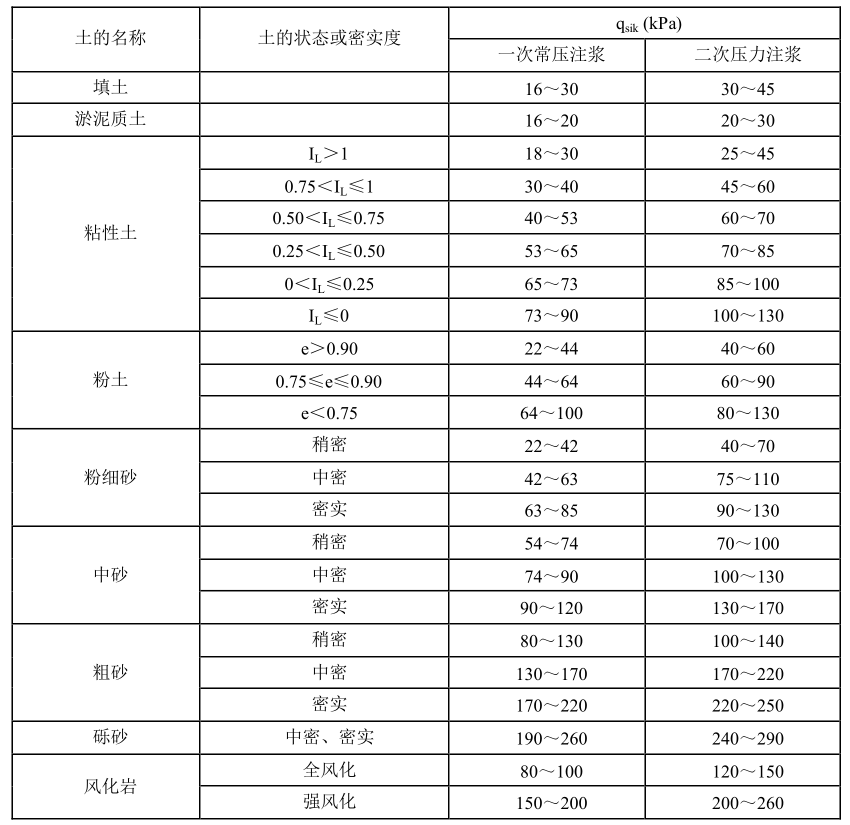
\includegraphics[width=0.8\linewidth]{figure/c8f3.png}
    \caption{锚杆的极限粘结强度标准值}
    \label{fig:c8f3}
\end{figure}

\subsection{施工安全保障措施}

(1) 基坑周围要设置安全标志警戒,提示施工人员注意安全,进入施工现场时必须佩戴安全帽。

(2) 机械和电气设备,非操作人员严禁触碰,操作人员要经过培训并持有对应的操作证件之后才可以上岗操作,在不操作的时候要关闭机械和电气的电源总开关,
有锁的设备应该及时上锁。

(3) 现场所有的特种设备都应做好登记备案,有专人维护,记录,上岗人员必须通过国家的职业技能考试,获取特种作业操作证件后才可上岗,不同班次的特种作业人员交接工作时要做好记录。

(4) 每一个用电器都要有单独的电箱控制,并且都要有锁,不得随意移动电源箱,非操作人员禁止触碰。

(5) 钢板桩插打、拔出、基坑开挖等高风险操作必须有防护员和专职的安全员在现场监督并实施防护措施才可开工。

(6) 插打桩时必须严格按照既定的方案设置基坑边线,无关人员不得逾越边线,打桩需使用专业打桩机,且操作打桩机的必须为持证上岗的打桩机操作手,操作过程中操作手必须严格遵守指令员
下发的指令,按照指令进行施工,如遇指令错误、未接到指令、或指令不清晰时严禁采取任何动作,也不得擅自开工。

(7) 基坑开挖和结构支护应该逐步交替进行,基坑应该分层开挖,开挖过程中要边挖边监测,如遇严重变形、严重偏离,路基严重沉降应立即停止开挖,立即回填,随后立即通知路政部门或设备管理单位进行养护。

(8) 在基础施工期间如遇地下不明管道和管线时,应当及时与有关部门联系,确认做好防护工作获得审批后才可继续施工。在地下管道,地下线缆,光缆附近施工时,应先征得有关部门的同意后,备齐充足的抢修材料,且拟定应急方案后才可动工。

(9) 钻孔桩施工前,应事先做好场地布置、调度和施工场所的排水降水工作。

(10) 所有施工用车辆务必保持完好状态,使用前要进行调整调试确保施工有序进行,在人多车多,施工车辆和施工人员混行的地区,应当设立临时的交通指挥人员。

(11) 电力线路周围三米范围之内禁止挖坑、挖沟、取土,堆土等,如无法避免,应当符合相关的规范和要求。


